\section{Background Estimation}
\subsection{\texorpdfstring{QCD Background Estimation in $\tauTau$ Channel}{QCD Background Estimation in tau-tau Channel}}
\label{sect:bkg}

%In this section, data driven methods are applied to estimate the contribution of
 %  the main backgrounds in the signal region.

In QCD multi-jet events all tau candidates are misidentified as jets. Due to large cross
section and
the poor MC modeling of the tau misidentification rate from jets, the QCD multi-jet contribution in the signal regions is estimated from data using the ABCD" method.

This method indeed relies on different distributions of QCD
in the four exclusive regions labelled as A, B, C (the control regions) and D (the signal region) are defined in a two-dimensional plane as a function of uncorrelated discriminating variables.
In this case the number of QCD events in signal region D can be calculated from the number of QCD events in the control region A multiplied in the ratio of the number of QCD events in the control region C to QCD events in control region B$(T=C/B)$.Figure~\ref{fig:1QCDbg} 

\begin{figure}[htbp]
\centering
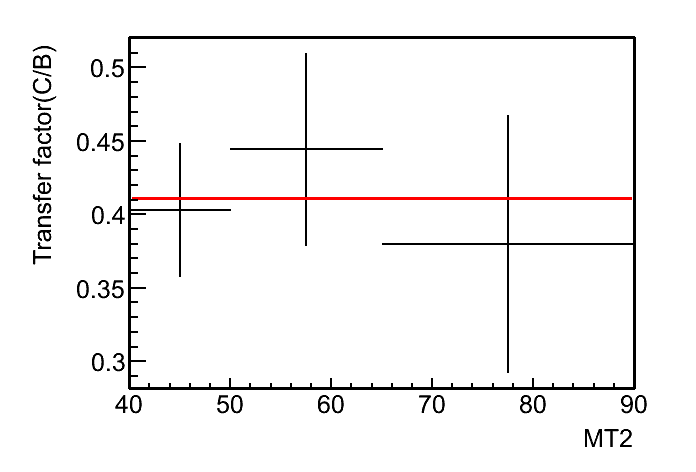
\includegraphics[width=0.49\textwidth]{QCDbginTauTau/Bin1_transferfactor.png}
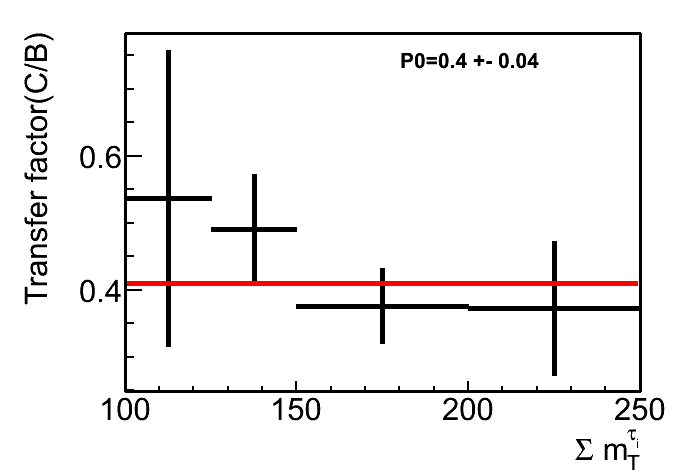
\includegraphics[width=0.49\textwidth]{QCDbginTauTau/Bin2_transferfactor.png} \\
\caption{The ratio of the number of QCD events in the control region C to QCD events in control region B.The
fit line  is drawn in red.
 Left:  $\mttwo>90$ Bin1   Right:  $\SumMT >250$ Bin2.}
\label{fig:1QCDbg}
\end{figure}

The tau identification criterion (tau-id) and a kinematic variable chosen depending (\mttwo in Bin 1 and \SumMT in Bin2) 
on the SR are used as the two uncorrelated discriminating variables to define the regions A, B, C and D. The definitions of the control regions are summarized in table \ref{2QCDbg}.

\begin{table}
\begin{center}
\begin{tabular}{|c|c|c|c|}
\hline
Region&A& B & C
\\ \hline\hline
$\mttwo>90$ Bin1 &$\mttwo >90$ & $\mttwo <90$&$\mttwo <90$ \\
 &at least 1 loose taus&at least 1 loose taus& loose tau veto\\
 &loose-loose loose-medium &loose-loose loose-medium &medium-medium \\
 &loose-tight&loose-tight&medium-tight tight-tight\\ 
 &No cut on charge&No cut on charge& Sum charge==0\\
\hline
$\SumMT>250$ Bin2 &$\SumMT >250$ &$\SumMT <250$&$\SumMT < 250$\\
 &at least 1 loose taus&at least 1 loose taus& loose tau veto\\
 &loose-loose loose-medium &loose-loose loose-medium &medium-medium \\
 &loose-tight&loose-tight&medium-tight tight-tight\\
 &No cut on charge&No cut on charge& Sum charge==0\\
% &misc.MinMetJetDphiPt40$>$1 is relaxed\\

\hline
\end{tabular}
\caption{The requirement on the kinematic variables used to define the control regions A,B,C.
$\mindphifour>1$ cut is relaxed. }
\label{2QCDbg}
\end{center}
\end{table}

The number of QCD multi-jet events in the control regions is estimated from data after subtraction of other SM contributions estimated from MC simulation.

In order to increase the data statistics, the cut on the $\mindphifour>1$ is relaxed.This cut was
introduced to suppress the QCD background events,now that we want to estimate QCD multi-jet background this cut is relaxed  .The only the ratio this efficiency should be
applied into account QCD in the control regions to estimate the number of QCD events in the signal region.

The fraction of QCD events with all selection cuts with respect to the QCD events with all selection cuts but the
$\mindphifour>1$ are shown in Figure~\ref{fig:3QCDbg} .

\begin{figure}[htbp]
\centering
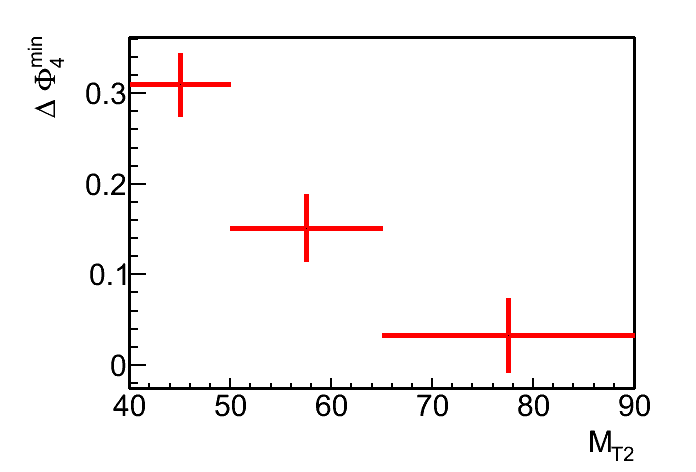
\includegraphics[width=0.49\textwidth]{QCDbginTauTau/Bin1_miscefficiency.png}
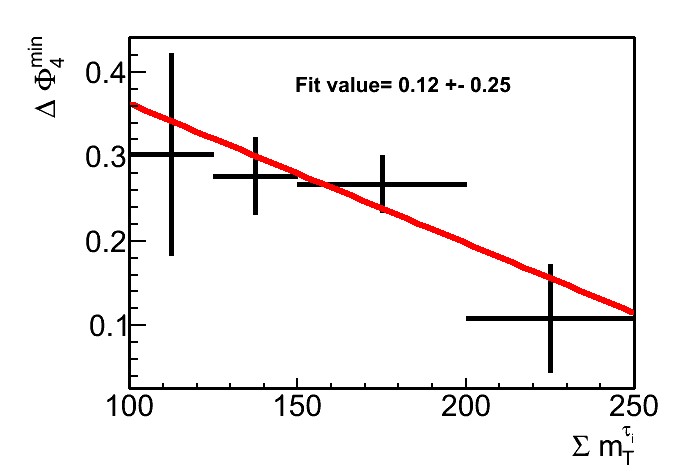
\includegraphics[width=0.49\textwidth]{QCDbginTauTau/Bin2_miscefficiency.png} \\
\caption{ Ratio between QCD multi-jet events passing all selection cuts versus QCD events
 passing all selection cuts but $MinMetJetDphiPt40>1$. Left:  $\mttwo>90$ Bin1   Right:  $\SumMT >250$ Bin2.}
\label{fig:3QCDbg}
\end{figure}




The results of the ABCD method are summarized in table \ref{4QCDbg} and the distributions of the kinematic variables  for data, SM backgrounds and SUSY are shown in the Figure~\ref{fig:5QCDbg}. The SM background distributions
are taken from MC simulation, except for the QCD-multi-jet contribution, which is estimated
using the ABCD method.



\begin{table}
\begin{center}
\scalebox{0.92}{
\begin{tabular}{|l|c|c|c|c|c|c|c|}
\hline
 & Sample & RegionA & RegionB & RegionC & T=C/B & QCD in Signal
 Region(D)\\
\hline\hline
\multirow{7}{*}{\mttwo$>$90}& Data&10.00 +- 3.16 & 880.00 +- 29.66&  430.00 +- 20.74& \multirow{7}{*}{0.43+-0.32} & \multirow{7}{*}{0.06 +- 0.08}\\ \cline{2-5}

&Z+jets& 2.27 +- 0.90 &29.27 +- 3.22 & 51.45 +- 4.43 & & \\\cline{2-5}

&W+jets& 2.90 +- 1.43&69.20 +- 8.70 &49.25 +- 7.22 & & \\\cline{2-5}

&WW+jets&0.12 +- 0.07 &0.76 +- 0.17 &1.60 +- 0.25 & & \\\cline{2-5}

&Top& 0.49 +- 0.47&21.78 +- 3.13 & 14.51 +- 2.63& & \\\cline{2-5}
&QCD& 4.23 +- 3.62 & 758.99+-31.24& 313.19+-22.55& & \\\cline{2-5}
&Susy& 1.46 +- 0.17& 3.96 +- 0.28& 9.01 +- 0.41& & \\\cline{2-5}
\hline\hline\hline
\multirow{7}{*}{$\SumMT>250$}&Data  &25.00 +- 5.00  &723.00 +- 26.89 &348.00 +- 18.65 & \multirow{7}{*}{ 0.41 +- 0.03} & \multirow{7}{*}{0.61 +- 1.55} &  \\
\cline{2-5}


&Z+jets& 2.22 +- 1.07 & 21.78 +- 2.72 & 39.57 +- 3.94& & \\\cline{2-5}

&W+jets&  4.28 +- 1.46&51.84 +- 7.48 & 40.09 +- 6.82& & \\\cline{2-5}

&WW+jets&  0.09 +- 0.05& 0.42 +- 0.13& 0.87 +- 0.19 & & \\\cline{2-5}

&Top&0.42 +- 0.41 &3.07 +- 1.22 & 3.31 +- 1.43& & \\\cline{2-5}
&QCD&18.00 +- 5.33 &645.89+-28.07 & 264.16+-20.30& & \\\cline{2-5}
&Susy& 2.13 +- 0.20&1.18 +- 0.15 &  2.80 +- 0.22& & \\\cline{2-5}
\hline\hline

\end{tabular}}
\caption{ The MC predicted backgrounds in the multi-jet control regions, including both the
statistical and systematic uncertainties, and the expected multi-jet contribution,obtained
by subtracting the MC contributions from observed data . Predicted event yields for the
SUSY  in the control regions are also shown. The estimated multi-jet contribution
in the SRs is given in the last column.
}
\label{4QCDbg}
\end{center}
\end{table}


\begin{figure}[htbp]
\centering
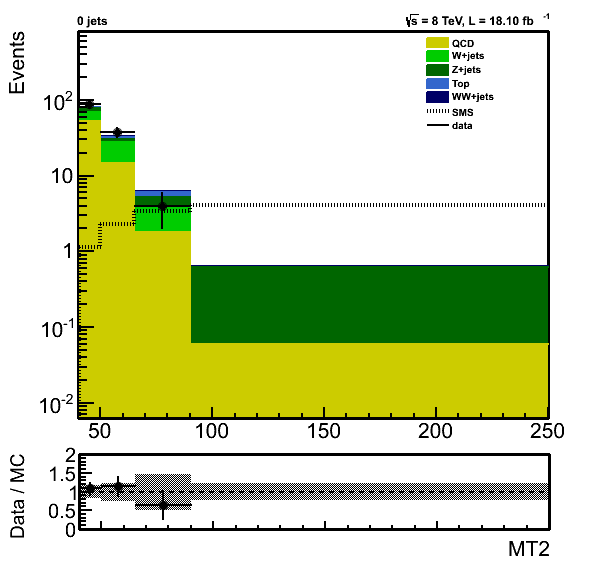
\includegraphics[width=0.49\textwidth]{QCDbginTauTau/Bin1_QCDdatadriven2.png}
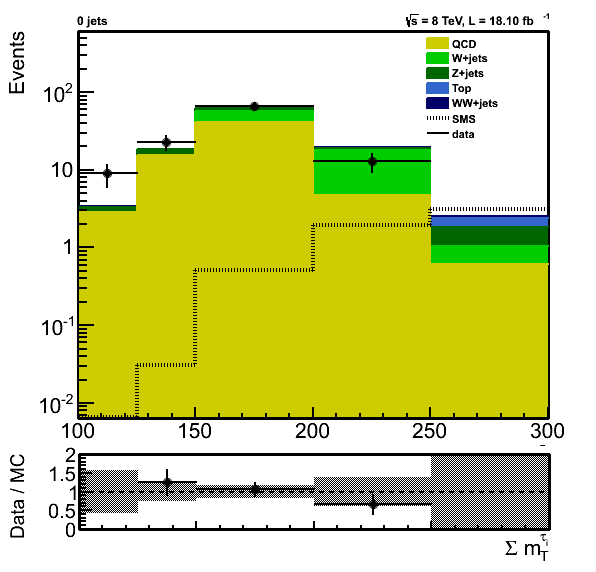
\includegraphics[width=0.49\textwidth]{QCDbginTauTau/Bin2_QCDdatadriven2.png} \\
\caption{Distributions of relevant kinematic variables before the requirement on the given variable
is applied: (a) \mttwo  (b) $\SumMT$ . The QCD multi-jet contribution is estimated from data using the ABCD method.}
\label{fig:5QCDbg}
\end{figure}

\subsection{\texorpdfstring{W+jets Background Estimation in $\tauTau$ Channel}{W+jets Background Estimation in tau-tau Channel}}
\subsubsection{Method Description}
As shown in the cut-flow-table, the number of W+jets events surviving the selection cuts are found to be zero in search bin\#1 or 0.43$\pm$0.40 in search bin\#2. In other words, due to the low statistics of W+jets events, the efficiency of $\mttwo$ is obtained to be zero, in bin\#1, or as found in bin\#2, the efficiency of $\SumMT$ is obtained very close to zero with a huge statistical uncertainty, namely 93\%. The statistical uncertainty on the yields for W+jets events can be improved by extracting the $\mttwo$ or $\SumMT$ cut efficieny, depending on the serach bins, in a sample with more statistics. This region is defined by relaxing some cuts which have marginal effects on either $\mttwo$ or $\SumMT$ variables. This way, the yields for W+jets events are reported with more statistical accuracy. In the next subsection, the validation of this method will be discussed.\\

\subsubsection{Method Validation}
Figure~\ref{fig:justification_bin1}  
\begin{figure}[htbp]
\centering
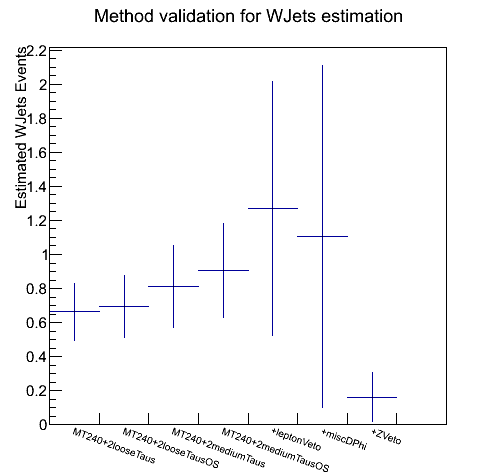
\includegraphics[angle=0,scale=0.35]{TauTauFigs/withMT2GT40.png}
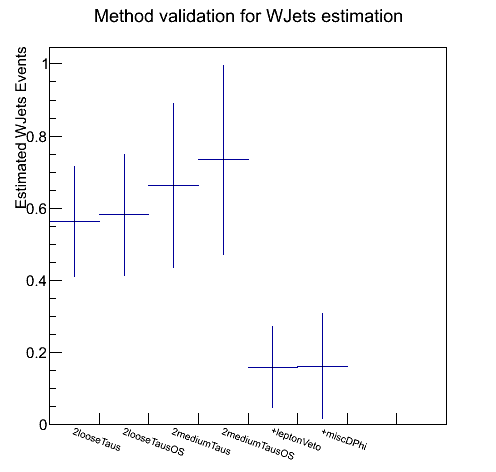
\includegraphics[angle=0,scale=0.35]{TauTauFigs/withMT2GT40ZVeto.png} \\
\caption{Cut efficiency for $\mttwo$ %(left) and \SumMT (right) 
in samples with various selections as labeled in each bin.}
\label{fig:justification_bin1}
\end{figure}
Figure~\ref{fig:justification_bin2}  
\begin{figure}[htbp]
\centering
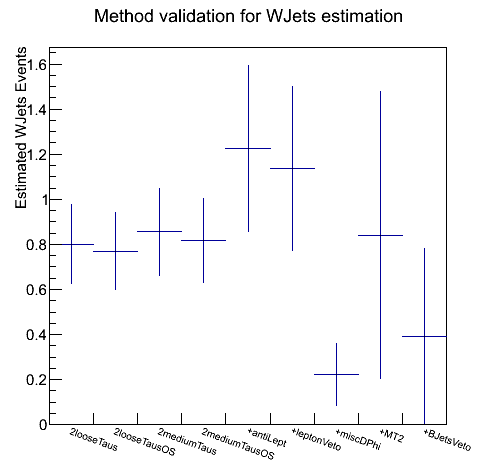
\includegraphics[angle=0,scale=0.35]{TauTauFigs/WJetsEst_bin2.png}
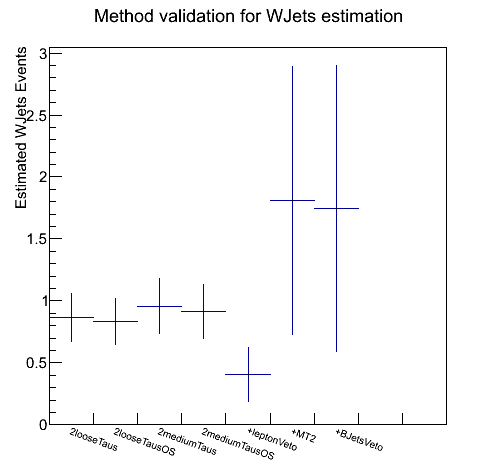
\includegraphics[angle=0,scale=0.35]{TauTauFigs/WJetsEst_bin2_miscApplied.png} \\
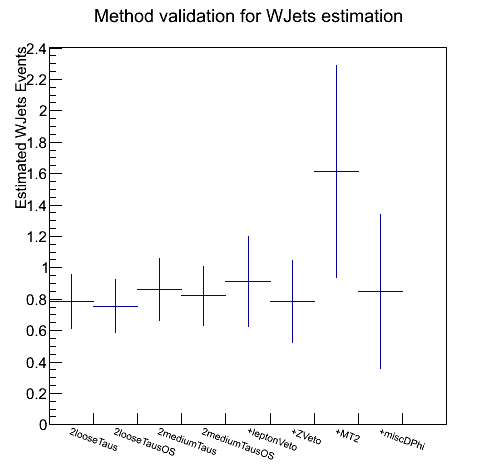
\includegraphics[angle=0,scale=0.35]{TauTauFigs/WJetsEst_bin2_BJetVetoApplied.png} \\
\caption{Cut efficiency for %\mttwo (left) and 
$\SumMT$ %(right) 
in samples with various selections as labeled in each bin.}
\label{fig:justification_bin2}
\end{figure}
\subsection{\texorpdfstring{DY Background Estimation in $\tauTau$ Channel}{DY Background Estimation in tau-tau Channel}}
\subsubsection{Method Description}
\subsubsection{Method Validation}
\subsection{\texorpdfstring{Fake Background Estimation in $\leptonTau$ Channel}{Fake Background Estimation in lepton-tau Channel}}
\label{sect:bkgLeptau}
In the $e/\mu-\hadtau$ channels, the main background is the W +jets, when the $\W$ boson decays to a lepton and a jet fakes a hadronic $\tau$.
We use a fake rate method to estimate this background \cite{CMS_AN_2010-261}. 
The idea is that when the loose signal selection is applied, the number of the loose $\hadtau$'s (L) is:
\begin{equation}
L = P + F
\end{equation}
P is the number of the  prompt $\hadtau$'s and F is the number of the  fake $\hadtau$'s. If the selection is tightened, the number of the tight $\hadtau$'s (T) is:
\begin{equation}
 T = pP + fF
\end{equation} 
p (f) is the prompt (fake) rate, the probablity that a loosely selected prompt (fake) $\hadtau$ can pass the  tight  selection. The loose category (L) can be divided to two parts, 
tight (T) and non-tight (NT), so one can write:
\begin{equation}
   F * (f - p) = ((1 - p) * L - NT)
\end{equation}
f * F is the contamination of the fake $\hadtau$'s in the signal region. 

The fake rate ({\it f}) is measured as the ratio of the tightly selected $\hadtau$'s to the loosely 
selected $\hadtau$'s in a sample which is dominated by the fake $\hadtau$'s. The fake rate is estimated in an environment which is as similar as possible to 
the signal region. The datasets and the triggers which are used to estimate the fake rate in different channels are shown in 
table \ref{Tab.DataFR}.
\begin{table}[!htb]
\begin{center}
\caption{The datasets and triggers for fake rate estimation.}
\label{Tab.DataFR}
\begin{tabular}{|l|c|c|}
\hline
Channel      & Data Set                                     & Trigger \\\hline
Muon Tau     & /SingleMu/Run2012D-22Jan2013-v1/AOD          & HLT\_IsoMu24\_v(16-17)\\
             &                                              & HLT\_IsoMu24\_eta2p1\_v(14-15)\\\hline
Electron Tau & /SingleElectron/Run2012D-22Jan2013-v1/AOD    & HLT\_Ele27\_WP80\_v11\\
\hline
\end{tabular}
\end{center}
\end{table}

%In the muTau channel, exactly one muon is required which passes the selection criteria of the muon in the signal region and has \pt > 27 GeV. 
Lepton selection and extra lepton rejections are exactly same as the signal selection. Only the \pt of the favorite lepton is forced to 
be 3 \GeV higher than the online cut resulting to \pt $>$ 27 \GeV for muon and \pt $>$ 27 \GeV for electron.
The rejections can reduce the contribution of the VV, DY and $\ttbar$ events. To further suppress the $\ttbar$ contamination, the b-veto 
similar to the signal selection is applied. The \MET is asked to be greater than 30 GeV, similar to the preselections. The selection of the $\hadtau$ is 
exactly same as the signal selection, except the $\hadtau$ isolation which is {\it Loose} for the loosely selected $\hadtau$'s and {\it Tight} for the 
tightly selected $\hadtau$'s.
The ratio of these two categories determines the fake rate. To avoid any bias from the trigger, the $\hadtau$'s closer than $\Delta$R = 0.2 to the 
lepton are rejected. 
The fake rate can be measured in the bins of $\hadtau$ \pt and $\eta$, but it is observed that the dependency is very small and can be ignored, 
so we use a single value for the fake rate which is XXXX +- XXX.

The prompt rate (p) is measured in the MC DY events. All of the preselections except the Z-veto and $\hadtau$ isolation are applied. The $\hadtau$ isolation 
is relaxed from {\it Tight} to {\it Loose}. Only the events that a generated $\tau$ decays hadronically are considered. If a reconstructed $\hadtau$ is 
closer than $\Delta R = 0.1$ to the generated $\tau$, it is selected. Among these $\hadtau$'s, the prompt rate is defined as the fraction of the loose $\hadtau$'s 
which are tight. The prompt rate can be measured in the bins of \mttwo, but the statistics in the high \mttwo region which is our favorite 
region is too low that we can not conclude anything about the shape of the prompt rate in this region, so we choose it as a constant value
XXXX +- XX in the whole \mttwo region.



